\chapter{Implementation}

\section{Verbatim text}

Verbatim text can be included using \verb|\begin{verbatim}| and
\verb|\end{verbatim}|. I normally use a slightly smaller font and
often squeeze the lines a little closer together, as in:

{\renewcommand{\baselinestretch}{0.8}\small
\begin{verbatim}
GET "libhdr"

GLOBAL { count:200; all  }

LET try(ld, row, rd) BE TEST row=all
                        THEN count := count + 1
                        ELSE { LET poss = all & ~(ld | row | rd)
                               UNTIL poss=0 DO
                               { LET p = poss & -poss
                                 poss := poss - p
                                 try(ld+p << 1, row+p, rd+p >> 1)
                               }
                             }
LET start() = VALOF
{ all := 1
  FOR i = 1 TO 12 DO
  { count := 0
    try(0, 0, 0)
    writef("Number of solutions to %i2-queens is %i5*n", i, count)
    all := 2*all + 1
  }
  RESULTIS 0
}
\end{verbatim}
}

\section{Tables}

\begin{samepage}
Here is a simple example\footnote{A footnote} of a table.

\begin{center}
\begin{tabular}{l|c|r}
Left      & Centred & Right \\
Justified &         & Justified \\[3mm]
%\hline\\%[-2mm]
First     & A       & XXX \\
Second    & AA      & XX  \\
Last      & AAA     & X   \\
\end{tabular}
\end{center}

\noindent
There is another example table in the proforma.
\end{samepage}

\section{Simple diagrams}

Simple diagrams can be written directly in \LaTeX.  For example, see
figure~\ref{latexpic1} on page~\pageref{latexpic1} and see
figure~\ref{latexpic2} on page~\pageref{latexpic2}.

\begin{figure}
\setlength{\unitlength}{1mm}
\begin{center}
\begin{picture}(125,100)
\put(0,80){\framebox(50,10){AAA}}
\put(0,60){\framebox(50,10){BBB}}
\put(0,40){\framebox(50,10){CCC}}
\put(0,20){\framebox(50,10){DDD}}
\put(0,00){\framebox(50,10){EEE}}

\put(75,80){\framebox(50,10){XXX}}
\put(75,60){\framebox(50,10){YYY}}
\put(75,40){\framebox(50,10){ZZZ}}

\put(25,80){\vector(0,-1){10}}
\put(25,60){\vector(0,-1){10}}
\put(25,50){\vector(0,1){10}}
\put(25,40){\vector(0,-1){10}}
\put(25,20){\vector(0,-1){10}}

\put(100,80){\vector(0,-1){10}}
\put(100,70){\vector(0,1){10}}
\put(100,60){\vector(0,-1){10}}
\put(100,50){\vector(0,1){10}}

\put(50,65){\vector(1,0){25}}
\put(75,65){\vector(-1,0){25}}
\end{picture}
\end{center}
\caption{A picture composed of boxes and vectors.}
\label{latexpic1}
\end{figure}

\begin{figure}
\setlength{\unitlength}{1mm}
\begin{center}

\begin{picture}(100,70)
\put(47,65){\circle{10}}
\put(45,64){abc}

\put(37,45){\circle{10}}
\put(37,51){\line(1,1){7}}
\put(35,44){def}

\put(57,25){\circle{10}}
\put(57,31){\line(-1,3){9}}
\put(57,31){\line(-3,2){15}}
\put(55,24){ghi}

\put(32,0){\framebox(10,10){A}}
\put(52,0){\framebox(10,10){B}}
\put(37,12){\line(0,1){26}}
\put(37,12){\line(2,1){15}}
\put(57,12){\line(0,2){6}}
\end{picture}

\end{center}
\caption{A diagram composed of circles, lines and boxes.}
\label{latexpic2}
\end{figure}



\section{Adding more complicated graphics}

The use of \LaTeX\ format can be tedious and it is often better to use
encapsulated postscript (EPS) or PDF to represent complicated graphics.
Figure~\ref{epsfig} and~\ref{xfig} on page \pageref{xfig} are
examples. The second figure was drawn using \texttt{xfig} and exported in
{\tt.eps} format. This is my recommended way of drawing all diagrams.


\begin{figure}[tbh]
\centerline{
\includegraphics{figs/cuarms.pdf}}
\caption{Example figure using encapsulated postscript}
\label{epsfig}
\end{figure}

\begin{figure}[tbh]
\vspace{4in}
\caption{Example figure where a picture can be pasted in}
\label{pastedfig}
\end{figure}


\begin{figure}[tbh]
\centerline{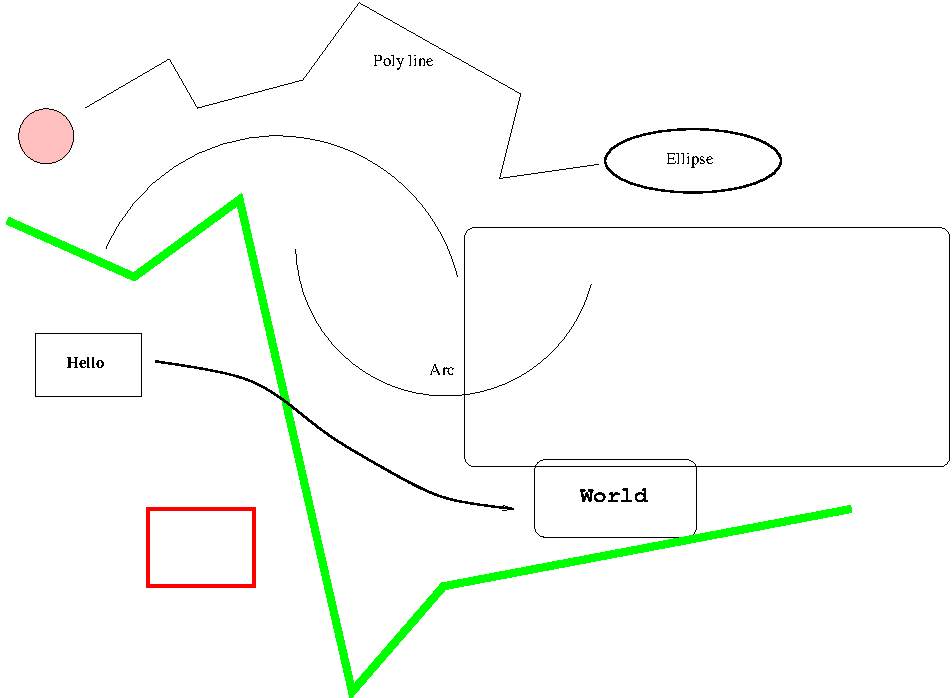
\includegraphics{figs/diagram.pdf}}
\caption{Example diagram drawn using \texttt{xfig}}
\label{xfig}
\end{figure}
